\Chapter{Megvalósítás}

\Section{Algoritmizálás}

\SubSection{Osztálydefiníciók}

\begin{python}
	class Room:
	def __init__(self, name, capacity, subjects):
	self.name = name
	self.capacity = capacity
	self.subjects = subjects
	
	
	class Teacher:
	def __init__(self, name, subjects, balance, extremisms, begin_time,
	end_time):
	self.name = name
	self.subjects = subjects
	self.balance = balance
	self.extremisms = extremisms
	self.begin_time = begin_time
	self.end_time = end_time
	
	
	class SimpleGroup:
	def __init__(self, name, grade, subjects, headcount):
	self.name = name
	self.grade = grade
	self.subjects = []
	for subject_name, subject_data in subjects.items():
	subject = Subject(subject_name, **subject_data)
	self.subjects.append(subject)
	self.room = ""
	self.headcount = headcount
	
	
	class Subject:
	def __init__(self, name, type, weekly_periods):
	self.name = name
	self.type = type
	self.weekly_periods = weekly_periods
	
	
	class Group:
	def __init__(self, name, grade, subject, type, weekly_periods,
	headcount):
	self.name = name
	self.grade = grade
	self.subject = subject
	self.type = type
	self.weekly_periods = weekly_periods
	self.room = ""
	self.teacher = ""
	self.headcount = headcount
\end{python}

Legelőször az osztálydefiníciókat láthatjuk. Mint már tudjuk, 4 tényezőnk van az órarendgenerálással kapcsolatban, viszont az osztályok kezelése kétféleképpen történik. A teremhozzárendelési feladat első fázisában még az eredeti formában (\textit{simple\_group}) kezeljük őket, utána viszont már "táblázatos" formában (\textit{group}). Hogy utóbbi mit jelent, azt korábban már kifejtettem.

\SubSection{Teremhozzárendelési feladat}

\begin{python}
	pairings = [[] for _ in range(len(simple_groups))]
	idles = [[] for _ in range(len(simple_groups))]
	for simple_group in range(len(simple_groups)):
	for room in range(len(rooms)):
	if simple_groups[simple_group].headcount <= rooms[room].capacity:
	pairings[simple_group].append(1)
	idles[simple_group].append(rooms[room].capacity -
	simple_groups[simple_group].headcount)
	else:
	pairings[simple_group].append(0)
	idles[simple_group].append(math.nan)
	
	seated_rooms = []
	seated_types = []
	for simple_group in range(len(simple_groups)):
	min = math.inf
	minindex = math.nan
	type = ""
	for room in range(len(rooms)):
	ok = False
	if (pairings[simple_group][room] == 1) and\
	(idles[simple_group][room] < min):
	for seated_room in range(len(seated_rooms)):
	if (rooms[room] == seated_rooms[seated_room]) and\
	(simple_groups[simple_group].subjects[0].type ==
	seated_types[seated_room]):
	ok = True
	break
	if not ok:
	min = idles[simple_group][room]
	minindex = room
	type = simple_groups[simple_group].subjects[0].type
	simple_groups[simple_group].room = rooms[room]
	if room == len(rooms) - 1:
	seated_rooms.append(rooms[minindex])
	seated_types.append(type)
\end{python}

A teremhozzárendelési feladat első fázisa két algoritmusból áll. Az első elkészíti azt a párosításmátrixot, amely minden terem és minden osztály esetében rögzíti, hogy az adott osztály befér-e az adott terembe és ha igen, mennyi lesz a kihasználatlanság. A második algoritmus már a hozzárendeléseket végzi el a párosításmátrix eredményeit felhasználva, optimálisan, azt is figyelembe véve, hogy az egyes osztályok alaposztályok vagy nyelvi, fakutációs, egyéb osztályok. Ugyanis egy alaposztály és egy, az évfolyamon képzett nyelvi, fakultációs vagy egyéb osztály beosztható ugyanabba a terembe.

\begin{python}
	def createTable(groups):
	rows = []
	for group in groups:
	for subject in group.subjects:
	row = Group(group.name, group.grade, subject.name,
	subject.type, subject.weekly_periods, group.headcount)
	rows.append(row)
	return rows
	
	
	groups = createTable(simple_groups)
	for simple_group in range(len(simple_groups)):
	for group in range(len(groups)):
	if groups[group].name == simple_groups[simple_group].name:
	ok = False
	for subject in range(len(simple_groups[simple_group].
	room.subjects)):
	if groups[group].subject ==\
	simple_groups[simple_group].room.subjects[subject]:
	ok = True
	break
	if not ok:
	ok = True
	for room in range(len(rooms)):
	for subject in range(len(rooms[room].subjects)):
	if groups[group].subject ==\
	rooms[room].subjects[subject]:
	ok = False
	break
	counter = 0
	if not ok:
	paired = False
	while not paired and counter != 10000:
	counter += 1
	rand_room = rooms[random.randint(0, len(rooms) - 1)]
	for subject in range(len(rand_room.subjects)):
	if (groups[group].subject ==
	rand_room.subjects[subject]) and\
	(groups[group].headcount <= 
	rand_room.capacity):
	groups[group].room = rand_room.name
	paired = True
	break
	if ok or counter == 10000:
	groups[group].room = simple_groups[simple_group].room.name
\end{python}

A teremhozzárendelési feladat második fázisában a \textit{createTable()} metódus segítségével a \textit{simple\_group} típusú osztály objektumainkat \textit{group} típusúakká alakítjuk, majd minden osztály esetében végignézzük az összes hozzá tartozó tantárgyat. Ha találunk olyan tárgya(ka)t, mely(ek)hez van "speciális" terem/termek, de az első fázis során hozzárendelt terem nem ilyen, akkor az osztály úgymond költözni fog az adott tantárgy kapcsán (vagyis az adott osztály-tantárgy kettőshöz másik terem rendelődik hozzá). Kivéve ha nagyobb a létszámuk minden ilyen terem befogadóképességénél, ez esetben maradnak az eredetileg hozzárendelt teremben (vagyis az adott osztály-tantárgy kettőshöz ugyanazt a termet rendeljük hozzá).

\SubSection{Tanárhozzárendelési feladat}

\begin{python}
	pairings = [[] for _ in range(len(groups))]
	for group in range(len(groups)):
	for teacher in range(len(teachers)):
	for subject in range(len(teachers[teacher].subjects)):
	if groups[group].subject ==\
	teachers[teacher].subjects[subject]:
	pairings[group].append(1)
	break
	elif subject == len(teachers[teacher].subjects) - 1:
	pairings[group].append(0)
	
	sum_periods = [0] * len(teachers)
	for group in range(len(groups)):
	for teacher in range(len(teachers)):
	if pairings[group][teacher] == 1:
	paired = True
	for other_teacher in range(teacher, len(teachers)):
	if (sum_periods[other_teacher] < 
	sum_periods[teacher]) and\
	(pairings[group][other_teacher] == 1):
	paired = False
	break
	if paired:
	groups[group].teacher = teachers[teacher].name
	sum_periods[teacher] += groups[group].weekly_periods
	break
\end{python}

Következő a tanárhozzárendelési feladat. Először itt is egy párosításmátrixot készítünk el, ami ezúttal tanárokat és osztály-tantárgy kettősöket vizsgál. Végigmegyünk a tanárok \textit{subjects} nevű, tömb típusú attribútumának elemein és ha találunk köztük olyat, ami megegyezik az adott osztály-tantárgy kettős tantárgy attribútumának értékével, akkor 1 kerül a "rublikába", ellenkező esetben 0.
A második algoritmus elvégzi a hozzárendeléseket, két dolgot vizsgálva. Az egyik a párosításmátrix értéke az adott tanár és osztály-tantárgy kettős viszonylatában, ami mindenféleképpen 1 kell, hogy legyen, a másik pedig, hogy van-e olyan másik tanár, aki szintén tudja tanítani az adott tárgyat és a heti óraszámának aktuális értéke kisebb. Ha nincs ilyen, akkor megtaláltuk azt a tanárt, akinek hozzárendelése optimális eredményre vezet az egyes tanárok terhelése közti különbségek minimalizálása kapcsán. Ez esetben hozzárendeljük őt az osztály-tantárgy kettőshöz.

\SubSection{Időablakok beosztása}

\begin{python}
	DAILY_PERIODS = end_time - begin_time
	NUM_TIME_WINDOWS = DAILY_PERIODS * 5
	
	
	def getPeriod():
	period = {'day': "", 'period': "", 'assignments': []}
	seated_groups = []
	viewed_groups = []
	for _ in range(len(teachers)):
	while True:
	if len(viewed_groups) == len(groups):
	return period
	rand = random.randint(0, len(groups) - 1)
	rand_group = groups[rand]
	ok = False
	for viewed_group in range(len(viewed_groups)):
	if rand == viewed_groups[viewed_group]:
	ok = True
	break
	if not ok:
	viewed_groups.append(rand)
	if sum_periods[rand] < rand_group.weekly_periods:
	ok = True
	for seated_group in range(len(seated_groups)):
	if (rand_group.name ==
	seated_groups[seated_group].name) or\
	(rand_group.grade == 
	seated_groups[seated_group].grade and
	rand_group.type != 
	seated_groups[seated_group].type):
	ok = False
	break
	elif rand_group.room ==\
	seated_groups[seated_group].room:
	ok = False
	break
	elif rand_group.teacher ==\
	seated_groups[seated_group].teacher:
	ok = False
	break
	if ok:
	seated_groups.append(rand_group)
	sum_periods[rand] += 1
	period['assignments'].append(rand_group)
	break
	return period
	
	
	sum_periods = [0] * len(groups)
	periods = []
	for period in range(NUM_TIME_WINDOWS):
	periods.append(getPeriod(groups, teachers, sum_periods))
\end{python}

Következő az időablakok beosztása. Itt már előre definiált konstansok is vannak. A felhasználó adja meg, hogy mettől meddig terjedjenek a napi időintervallumok, amely értékek a \textit{begin\_time} és \textit{end\_time} változókban adódnak át. Pl. ha reggel 7 és délután 4 óra között van tanítás az egyes napokon, akkor a \textit{begin\_time} 7, az \textit{end\_time} pedig 16 lesz, a \textit{DAILY\_PERIODS} konstans pedig a kettő különbségeként 9, ennyi időablak lesz egy napon. A \textit{NUM\_TIME\_WINDOWS} a heti összes időablak száma, ami így ennek ötszöröse, a \textit{MAX\_ASSIGNMENTS} által pedig azt rögzítjük, legfeljebb hány osztály-tantárgy-terem-tanár hozzárendelés lehet egy időablakban, ami a tanárok számával lesz megegyező. A lényegi részt a \textit{getPeriod()} metódus adja, ami két feltételnek eleget tevő megoldást szolgáltat. Az egyik az ütközésmentesség, vagyis hogy egy időablakban ugyanaz az osztály, ugyanaz a terem és ugyanaz a tanár sem fordulhat elő többször, sőt egy alaposztály és annak évfolyamán képzett nyelvi, fakultációs vagy egyéb osztály, illetve utóbbiak közül egyszerre több sem kerülhet ugyanabba az időablakba. A másik, hogy egy osztály-tantárgy kettősnek annyiszor kell összesen előfordulnia, amennyi a rögzített heti óraszáma az adott osztálynak az adott tárgyból. Ezt a \textit{getPeriod()} metódust aztán annyiszor hívjuk meg, amennyi a heti összes időablak száma. Az, hogy ez elegendő legyen, vagyis minden tanórának jusson időablak, a felhasználó felelőssége.

\SubSection{Időintervallumok hozzárendelése genetikus algoritmussal}

\begin{python}
	SIZE_POPULATION = 100
	CROSSOVER_RATE = 80
	MUTATION_RATE = 5
	SCALE_MAX = 5
	DAILY_PERIODS = end_time - begin_time
	NUM_GENS = DAILY_PERIODS * 5
	time_windows = {'m': [], 'tu': [], 'w': [], 'th': [], 'f': []}
	
	
	class Day(Enum):
	m = 0
	tu = 1
	w = 2
	th = 3
	f = 4
	
	
	for day in range(5):
	day = Day(day)
	counter = 0
	for period in range(DAILY_PERIODS):
	time_windows[day.name].append(begin_time + counter)
	counter += 1
\end{python}

Elérkeztünk az időintervallumok hozzárendeléséhez, genetikus algoritmus segítségével. Először a globális változók definiálását és a \textit{time\_windows} szótár feltöltését láthatjuk. A populáció létszámának, valamint a keresztezési és mutációs rátáknak a meghatározása tapasztalati úton történt, a \textit{SCALE\_MAX} azt rögzíti, hogy ötös skálán kell a felhasználónak megválasztani a tanárok \textit{balance} és \textit{extremisms} attribútumainak értékeit, a többi pedig már ezelőtt is előfordult. A \textit{time\_windows} szótár 5 tömböt tartalmaz, melyek a hét napjai, azok elemei pedig az időintervallumok. Azt, hogy hány eleműek ezek a tömbök és milyen időintervallumokat tartalmaznak, előzetesen nem tudni, így a lentebb található algoritmus fogja őket feltölteni, miután megvan a felhasználó által megadott \textit{begin\_time}, és az abból származtatott \textit{DAILY\_PERIODS} érték.

\begin{python}
	def getRandomGens():
	gens = {'days': [], 'periods': []}
	seated_windows = {'days': [], 'periods': []}
	for gen in range(NUM_GENS):
	ok = False
	rand_day = math.nan
	rand_period = math.nan
	while not ok:
	ok = True
	rand_day = random.randint(0, 4)
	rand_day = Day(rand_day)
	rand_period =\
	time_windows[rand_day.name][random.randint(0, 
	DAILY_PERIODS - 1)]
	for seated_window in range(len(seated_windows['days'])):
	if (rand_day.name ==
	seated_windows['days'][seated_window]) and\
	(rand_period == 
	seated_windows['periods'][seated_window]):
	ok = False
	break
	gens['days'].append(rand_day.name)
	gens['periods'].append(rand_period)
	seated_windows['days'].append(rand_day.name)
	seated_windows['periods'].append(rand_period)
	return gens
\end{python}

A \textit{getRandomGens()} metódus annyiszor megy végig ciklusban, amennyi az egyed génjeinek száma, ami a heti összes időablak száma. Minden génhez (időablakhoz) generál véletlenszerűen egy napot és egy, a napon belüli időintervallumot, nyilván ismétlődés nélkül. Ezáltal az egyedek a \textit{gens} változójukban véletlenszerű sorrendben fogják tartalmazni az időintervallumokat.

\begin{python}
	def targetFunction(entity):
	diff = 0
	for period in range(NUM_GENS):
	if entity['gens']['days'][period] == "f":
	diff += balance * len(periods[period]['assignments']) * 2
	if entity['gens']['periods'][period] == time_windows['f'][0]:
	diff += (SCALE_MAX - extremisms + 1) *\
	len(periods[period]['assignments']) * 2
	elif entity['gens']['periods'][period] == time_windows['f'][1]:
	diff += (SCALE_MAX - extremisms + 1) * len(periods[period]['assignments'])
	elif entity['gens']['periods'][period] ==\
	time_windows['f'][DAILY_PERIODS - 1]:
	diff += extremisms * len(periods[period]['assignments']) * 2
	elif entity['gens']['periods'][period] ==\
	time_windows['f'][DAILY_PERIODS - 2]:
	diff += extremisms * len(periods[period]['assignments'])
	return diff
\end{python}

\begin{python}
	def targetFunction(entity):
	diff = 0
	for teacher in range(len(teachers)):
	for period in range(NUM_GENS):
	for assignment in range(len(periods[period]['assignments'])):
	if periods[period]['assignments'][assignment].teacher ==\
	teachers[teacher].name:
	if entity['gens']['days'][period] == "f":
	diff += teachers[teacher].balance *\
	len(periods[period]) * 2
	if entity['gens']['periods'][period] ==\
	time_windows['f'][0]:
	diff += (SCALE_MAX -
	teachers[teacher].extremisms + 1) *\
	len(periods[period]) * 2
	elif entity['gens']['periods'][period] ==\
	time_windows['f'][1]:
	diff += (SCALE_MAX -
	teachers[teacher].extremisms + 1) *\
	len(periods[period])
	elif entity['gens']['periods'][period] ==\
	time_windows['f'][DAILY_PERIODS - 1]:
	diff += teachers[teacher].extremisms *\
	len(periods[period]) * 2
	elif entity['gens']['periods'][period] ==\
	time_windows['f'][DAILY_PERIODS - 2]:
	diff += teachers[teacher].extremisms *\
	len(periods[period])
	return diff
\end{python}

\begin{python}
	def targetFunction(entity):
	diff = 0
	for teacher in range(len(teachers)):
	for period in range(NUM_GENS):
	for assignment in range(len(periods[period]['assignments'])):
	if periods[period]['assignments'][assignment].teacher ==\
	teachers[teacher].name:
	if (entity['gens']['periods'][period] < 
	teachers[teacher].begin_time) or\
	(entity['gens']['periods'][period] > 
	teachers[teacher].end_time):
	diff += SCALE_MAX * 2
	if entity['gens']['days'][period] == "f":
	diff += teachers[teacher].balance *\
	len(periods[period]) * 2
	if entity['gens']['periods'][period] ==\
	time_windows['f'][0]:
	diff += (SCALE_MAX - 
	teachers[teacher].extremisms + 1) *\
	len(periods[period]) * 2
	elif entity['gens']['periods'][period] ==\
	time_windows['f'][1]:
	diff += (SCALE_MAX - 
	teachers[teacher].extremisms + 1) *\
	len(periods[period])
	elif entity['gens']['periods'][period] ==\
	time_windows['f'][DAILY_PERIODS - 1]:
	diff += teachers[teacher].extremisms *\
	len(periods[period]) * 2
	elif entity['gens']['periods'][period] ==\
	time_windows['f'][DAILY_PERIODS - 2]:
	diff += teachers[teacher].extremisms *\
	len(periods[period])
	return diff
\end{python}

Az, hogy a célfüggvény (\textit{targetFunction()} metódus) milyen előfordulásokat (vagy azok hiányát) "büntessen" és milyen súllyal, azt a programozó szabadon megválaszthatja, bármit bele lehet tenni. Az is megvalósítható, hogy a felhasználó eldönthesse, milyen tényezők érdeklik egyáltalán. Mint látható, 3-féle verziót készítettem. Az első verzió a kora reggeli/késő délutáni órák minimalizálását és a napi óraszámok arányos eloszlását/pénteki órák minimalizálását egységesen megadott/alapértelmezett súlyozással végzi. A másodiknál minden tanár esetén beállíthatja a felhasználó ötös skálán, milyen fontosak neki az egyes feltételek. Ezek az értékek adják ugye a súlyokat. Megemlítendő még, hogy a kora reggeli/késő délutáni órák minimalizálása kapcsán az adott napok első és második, valamint utolsó és utolsó előtti időintervallumánál is büntetőpontok járnak, az első és utolsó időintervallum esetében kétszeresen. A harmadik verzióban ezenkívül még a részmunkaidős tanárok olyan időintervallumokban való előfordulása is büntetést von maga után, amikor nem érnek rá. A futási idő egészen minimálisan lesz csak több a harmadik verzióban a másodikhoz képest, mert ugyanaz a ciklikus bonyolultság, ebből két következtetést vonhatunk le. Az egyik, hogy mivel ebben az esetben úgyis végig kell vizsgálni minden tanár előfordulását minden időintervallumban, így nyugodtan lehetnek tanáronkénti súlyok egységes helyett, a másik pedig, hogy mivel a második verzió esetében is végig kell vizsgálni, ezért nyugodtan hozzárakhatjuk a harmadik verzióban levő bővítést. Vagyis az első vagy a harmadik verziót érdemes használni. Végül még elmondhatjuk, hogy a lyukas órák számának minimalizálását a kora reggeli/késő délutáni órák számának minimalizálásával nagy mértékig elérjük, így kifejezetten erre irányuló eljárást, ami nagyon-nagyon megnövelné a futási időt, nem jó ötlet alkalmazni. A büntetőpont (\textit{diff}) aktuális értéke mindig úgy áll elő, hogy az adott időintervallumban levő osztály-tantárgy-terem-tanár hozzárendelések számát a megfelelő súllyal szorozzuk, ennyivel növeljük a büntetőpont értékét. Ha az összes időintervallumon végigmentünk az összes tanár esetében, a célfüggvény értéke előáll az adott egyed kapcsán. Ezután egy rendező metódus következik, ami a célfüggvény értékek alapján rendezi sorba az egyedeket, majd jöhet a második generáció kitenyésztése.

\begin{python}
	def selectParent(either_parent):
	while True:
	rand = random.randint(0, total - 1)
	for entity in range(SIZE_POPULATION):
	for weight in range(len(weights[entity])):
	if rand == weights[entity][weight]:
	if entities[entity]['id'] != either_parent['id']:
	return entities[entity]
\end{python}

A szelekciót biztosító metódus (\textit{selectParent()}) már a \textit{createChildren()} metódusból fog meghívásra kerülni. Véletlenszámot generál, melynek alsó határa 0, felső határa pedig a populáció létszámának a Fibonacci-száma (\textit{total}) - 1. A súlyozott randomgenerátor által, a rangsorban betöltött pozíciók alapján előállított \textit{weights} tömböket használja fel annak meghatározására, hogy az adott véletlenszám esetén melyik egyedet kapjuk meg, mint szülőt. Ugyanez a metódus meghívódik még egyszer, hiszen két szülője van egy gyereknek, ekkor ellenőrizni kell, hogy nehogy ugyanazt az egyedet válasszuk ki újra.

\begin{python}
	def createChildren(entity):
	either_parent = selectParent({'gens': {'days': [], 'periods': []}, 
		'diff': 0, 'id': entity})
	other_parent = selectParent(either_parent)
	order_crossover = random.randint(1, 100)
	if order_crossover > (100 - CROSSOVER_RATE):
	child = crossover(either_parent, other_parent)
	else:
	child = clear_inheritance(either_parent)
	order_mutation = random.randint(1, 100)
	if order_mutation > (100 - MUTATION_RATE):
	child = mutation(child)
	child['diff'] = targetFunction(child)
	return child
\end{python}

Miután megvan, kik lesznek a szülők, annak eldöntésére, hogy tiszta örökés legyen (az egyik szülő teljes génkészletének öröklése), keresztezés és/vagy mutáció, újabb véletlenszám generálásokra van szükség. A keresztezési ráta (\textit{CROSSOVER\_RATE}) és a mutációs ráta (\textit{MUTATION\_RATE}) értéke határozza meg a különböző esetek bekövetkezésének valószínűségét, melyek mind külön metóduson keresztül kerülnek megvalósításra.

\begin{figure}
	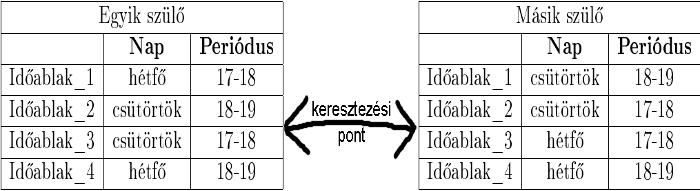
\includegraphics[width=\linewidth]{images/pelda.png}
	\caption{A keresztezés problematikája}
\end{figure}

\begin{table}
	\caption{Gyerek egyed}
	$$
	\begin{tabular}{|l|c|c|}
	\hline
	\multicolumn{3}{|c|}{Gyerek egyed}\\
	\hline
	& \bf{Nap} & \bf{Periódus}\\
	\hline
	Időablak\_1 & hétfő & 17-18\\
	\hline
	Időablak\_2 & csütörtök & 18-19\\
	\hline
	Időablak\_3 & hétfő & 17-18\\
	\hline
	Időablak\_4 & hétfő & 18-19\\
	\hline
	\end{tabular}
	$$
\end{table}

\begin{python}
	def crossover(either_parent, other_parent):
	child = {'gens': {'days': [], 'periods': []},
		'diff': 0, 'id': entity}
	crossover_point = random.randint(0, NUM_GENS - 1)
	for gen in range(0, crossover_point):
	child['gens']['days'].append(
	either_parent['gens']['days'][gen])
	child['gens']['periods'].append(
	either_parent['gens']['periods'][gen])
	for gen in range(crossover_point, NUM_GENS):
	ok = True
	for child_gen in range(len(child['gens']['days'])):
	if (child['gens']['days'][child_gen] ==
	other_parent['gens']['days'][gen]) and\
	(child['gens']['periods'][child_gen] ==
	other_parent['gens']['periods'][gen]):
	ok = False
	break
	if ok:
	child['gens']['days'].append(
	other_parent['gens']['days'][gen])
	child['gens']['periods'].append(
	other_parent['gens']['periods'][gen])
	else:
	for parent_gen in range(0, crossover_point):
	ok = True
	for child_gen in range(len(child['gens']['days'])):
	if (other_parent['gens']['days'][parent_gen] ==
	child['gens']['days'][child_gen]) and\
	(other_parent['gens']['periods'][parent_gen] ==
	child['gens']['periods'][child_gen]):
	ok = False
	break
	if ok:
	child['gens']['days'].append(
	other_parent['gens']['days'][parent_gen])
	child['gens']['periods'].append(
	other_parent['gens']['periods'][parent_gen])
	break
	return child
\end{python}

A keresztező metódus (operátor) még egy utolsó véletlenszám generálást végez, ami a keresztezési pont meghatározásához szükséges. A keresztezési pont előtt levő géneket az egyik szülő génkészletéből veszi át a gyermek, az utána levőket pedig a másik szülő génkészletéből, a normál egypontos keresztezési eljárásban. Itt a képeken látható problematika miatt egy speciálisabb, bonyolultabb eljárást kellett alkotni. A probléma arról szól, hogy ha egyszerűen csak átvesszük a szülő egyedek génjeit, jó eséllyel lesz olyan időintervallum (gén), ami kétszer is elő fog fordulni a gyerek génjei között, illetve ezzel együtt olyan, amelyik egyszer sem. A keresztezési pont után jelentkezik ez a probléma és úgy küszöböljük ki, hogy amennyiben már megtalálható a gyerek génjei között a szülő adott génje, akkor a szülő keresztezési pont előtti génjei között megkeressük az első olyat, amely még nem.

\begin{python}
	def clear_inheritance(either_parent):
	child = {'gens': {'days': [], 'periods': []}, 
		'diff': 0, 'id': entity}
	for gen in range(0, NUM_GENS):
	child['gens']['days'].append(either_parent['gens']['days'][gen])
	child['gens']['periods'].append(
	either_parent['gens']['periods'][gen])
	return child
\end{python}

Mint már mondtam, a tiszta öröklés esetében teljes mértékben az egyik szülő génállományát örökli a gyerek. További magyarázatot ez nem igényel.

\begin{python}
	def mutation(child):
	rand_entity = entities[random.randint(0, SIZE_POPULATION - 1)]
	muted_gen = random.randint(0, NUM_GENS - 1)
	for gen in range(0, NUM_GENS - 1):
	if (child['gens']['days'][gen] ==
	rand_entity['gens']['days'][NUM_GENS - 1]) and\
	(child['gens']['periods'][gen] ==
	rand_entity['gens']['periods'][NUM_GENS - 1]):
	child['gens']['days'][gen] ==\
	child['gens']['days'][muted_gen]
	child['gens']['periods'][gen] ==\
	child['gens']['periods'][muted_gen]
	child['gens']['days'][muted_gen] ==\
	rand_entity['gens']['days'][NUM_GENS - 1]
	child['gens']['periods'][muted_gen] ==\
	rand_entity['gens']['periods'][NUM_GENS - 1]
	break
	return child
\end{python}

A mutációs metódusban (operátorban) random generálunk egy mutálandó gént és egy idegen egyedet (vagyis olyan egyedet, aki nem szülője a gyereknek). Az idegen egyed sorrendileg utolsó génjének megfelelő gént megkeressük a gyerek génjei között, és azt felcseréljük a mutálandó génnel.

\begin{python}
	while True:
	new_entities = []
	for entity in range(SIZE_POPULATION):
	new_entities.append(createChildren(entity))
	entities = new_entities
	sortEntities()
	if entities[0]['diff'] - entities[SIZE_POPULATION - 1]['diff'] == 0:
	break
	
	for gen in range(NUM_GENS):
	periods[gen]['day'] = entities[0]['gens']['days'][gen]
	periods[gen]['period'] = entities[0]['gens']['periods'][gen]
\end{python}

A generációk száma előre nem meghatározott, mert a tesztelés során kiderült, hogy az egyedek célfüggvény értékei konvergálnak az optimumhoz (a minimális értékhez) és nem csak a legjobb egyed éri el, hanem mind. Ebből kifolyólag olyan feltételhez kötöttem a leállást, hogy a legjobb egyed célfüggvény értékének meg kell egyeznie a legrosszabb egyed célfüggvény értékével. Vagyis az összes egyed célfüggvény értékének megegyezőnek kell lenni. Végül beleírjuk a \textit{periods} listába a napokat és időintervallumokat, amire a \textit{generator.py}-nak szüksége lesz.

\Section{Adatbázis}

\begin{figure}
	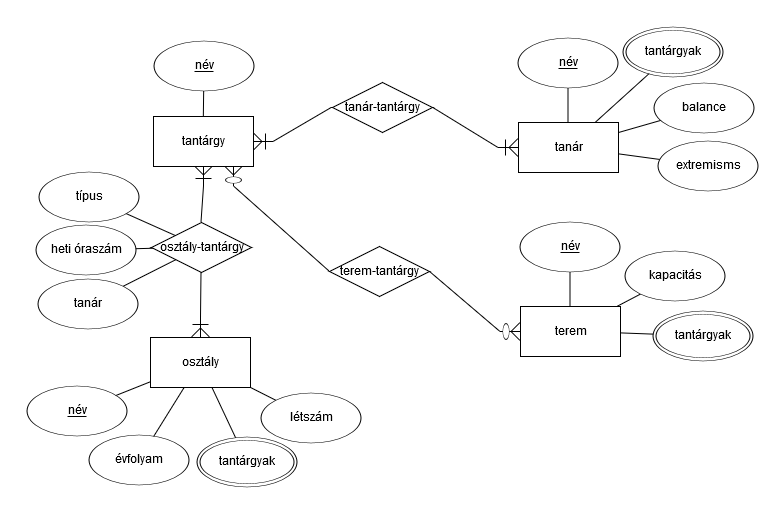
\includegraphics[width=\linewidth]{images/ermodell.png}
	\caption{Az ER modell}
\end{figure}

\begin{figure}
	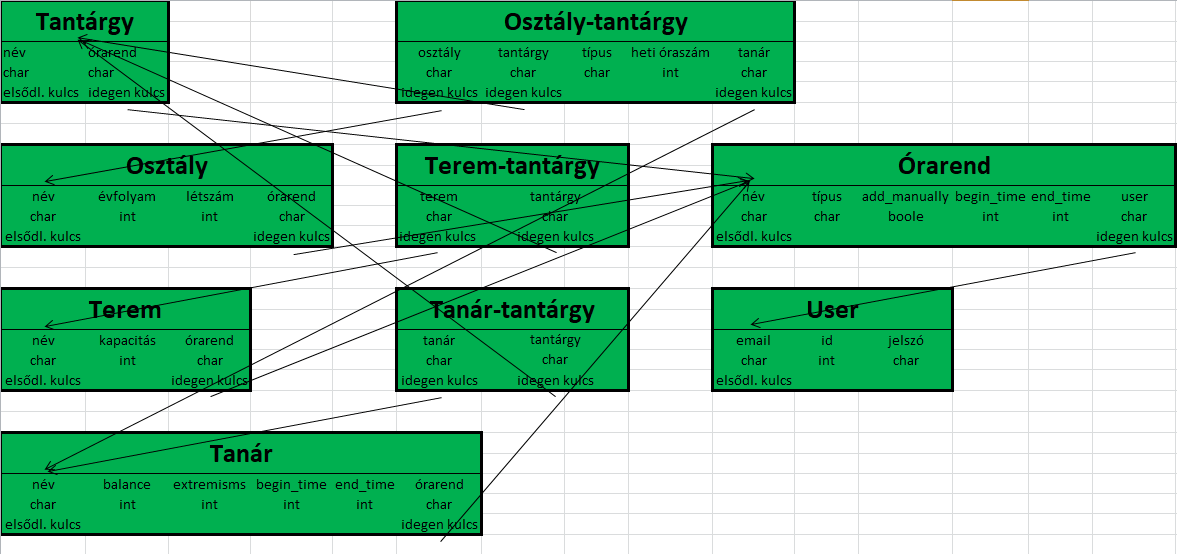
\includegraphics[width=\linewidth]{images/relmodell.png}
	\caption{A relációs modell}
\end{figure}

Adatbázist kellett használni a felhasználók által létrehozott órarendek adatainak a letárolásához és felhozásához. 6 entitásunk van (osztály, tantárgy, terem, tanár, órarend, felhasználó), de a több-több kapcsolatok miatt további táblákat is létre kellett hozni, a relációs modell már tartalmazza ezeket. 1:N kapcsolat van az osztály-tantárgy kapcsolótábla és a tanár tábla között, az órarend tábla és az osztály, tantárgy, tanár, terem táblák között, valamint az órarend és felhasználó tábla közt, a többi kapcsolat N:M (osztály-tantárgy, terem-tantárgy, tanár-tantárgy). A terem-tantárgy kapcsolatok opcionálisak, mert nem muszáj tantárgynak tartoznia egy adott teremhez, ahogyan egy adott tantárgyhoz sem muszáj, hogy tartozzon terem, a többi kapcsolat kötelező. A felhasználókat leszámítva minden entitás esetén a név szolgál egyedi azonosítóként, ami egyedül a tanárok esetén okozhatna problémát, de felhívjuk rá a felhasználó figyelmét, hogy azonos nevű tanárok esetén római számokkal való megkülönböztetést használjon, ezt elkerülendő. Python-ban az adatbázis tábláit osztályokként definiáljuk, ennek kapcsán kell még egy magyarázatot megtennem. Az osztály-tantárgy kapcsolótábla tanár idegen kulcsának értéke alapértelmezetten üres string. Ennek oka, hogy a felhasználó új órarend létrehozásakor eldöntheti, maunálisan akarja-e majd hozzárendelni az osztály-tantárgy kettősökhöz a tanárokat, amennyiben nem, akkor is léteznie kell ennek az attribútumnak, de addig üres string marad az értéke, amíg a tanárhozzárendelési algoritmus során kapott eredmények nem tárolódnak az adatbázisban, és a felhasználó által közvetlenül nem megváltoztatható.

\Section{Webalkalmazás}

Az egyoldalas webalkalmazás komponenseit vue fájlok alkotják, bennük egy html kódrésszel és egy script kódrésszel, amihez a Vue axios csomagját importáltam. A szkriptekben definiáltam az objektumokat (osztályok, tantárgyak, tantermek, tanárok és még többet is) a megfelelő adattagokkal és azokkal a metódusokkal, amelyek HTTP kéréseket intéznek a szerverhez (így közvetetten interakciót folytatnak az adatbázissal), illetve kliensoldali ellenőrzést végeznek. Ez utóbbira és a felhasználó által aktuálisan hozzáadott objektum példányok letárolására, illetve törlésre általam definiált metódust használtam, korábban eltárolt adatok felhozásához (bármely, de nem befoglaló objektum kapcsán) pedig a gyári \textit{created()} és \textit{mounted()} metódusokat definiáltam felül. Előbbi a komponens betöltésekor hívódik meg, utóbbi minden frissítéskor. A html kódrészben a Vue által biztosított módokon átadjuk az adatokat a megfelelő metódusnak (ezáltal "felvisszük" őket), vagy fogadjuk az adatokat a megfelelő metódustól és megjelenítjük.

A \textit{model.py} fájlban (ez egy Python modul) található az adatbázis tartalmának leképezése objektum-orientáltan, a \textit{timetable.py} HTTP kéréseket teljesítő metódusai ennek alapján tudnak az adatokra hivatkozni. Ezek a létrehozó, lekérdező, módosító, törlő metódusok mindig "ülést nyitnak", vagyis database session-t a \textit{database\_session.py} modul közbenjárásával, az adatbázishoz való hozzáféréshez. Ezenkívül egyes metódusok az adatok szerveroldali ellenőrzésére megírt metódust is meghívnak, melyeket szintén ebben a modulban definiáltam. A \textit{server.py} modulhoz futnak be a HTTP kérések a vue komponensekből, ugyanis ez a szerver. Ez a modul végzi el minden kérésnél az authentikációt, vagyis a felhasználói jogosultság ellenőrzését a token alapján, majd hívja meg a \textit{timetable.py} megfelelő metódusát, és a kapott eredményt vagy hibaértesítést aztán a HTTP protokoll szabványos formájában továbbítja a vue komponensnek. Itt használjuk fel a Falcon, a Waitress és a JWT nyújtotta szolgáltatásokat, melyeket röviden kifejtettem korábban.

Amikor a felhasználó már minden adatot felvitt és szeretné generáltatni az órarendeket, akkor a HTTP kérelem után, a \textit{server.py}-ból az adott órarendhez tartozó összes osztály, tantárgy, tanár, tanterem felhozásra kerül az adatbázisból, és ezúttal nem adjuk vissza a vue komponensnek json-ben, hanem eredeti formátumban a \textit{generator.py} számára továbbítjuk őket. A \textit{generator.py} először objektumokat példányosít a beérkezett szótár típusú adatokból, majd ezeket paraméterként átadja az órarendgenerálási részfeladatokat elvégző modulok globális metódusainak. Utána összegyűjti az adott osztályokhoz, tanárokhoz, illetve tantermekhez tartozó hozzárendeléseket, majd rendezi őket, úgy hogy a hétfői nap legkorábbi időintervalluma legyen a lista első és a pénteki nap legutolsó időintervalluma az utolsó eleme. Legvégül átadja az eredményeket az \textit{exporter.py}-nak. Az \textit{exporter.py} felelős a fájlok létrejöttéért és tartalommal való feltöltéséért. Utóbbit a Jinja segítségével valósítja meg, amely segít az eredmények html fájlokba való beleírásában. Ehhez egy \textit{template.html} nevű sablont készítettem, ami alapján a megadott helyekre a különböző osztályok, tanárok, tantermek kapcsán aktuális adatok fognak íródni. Végül Pandoc segítségével a html-eket pdf-ekké konvertáljuk.

\begin{figure}
	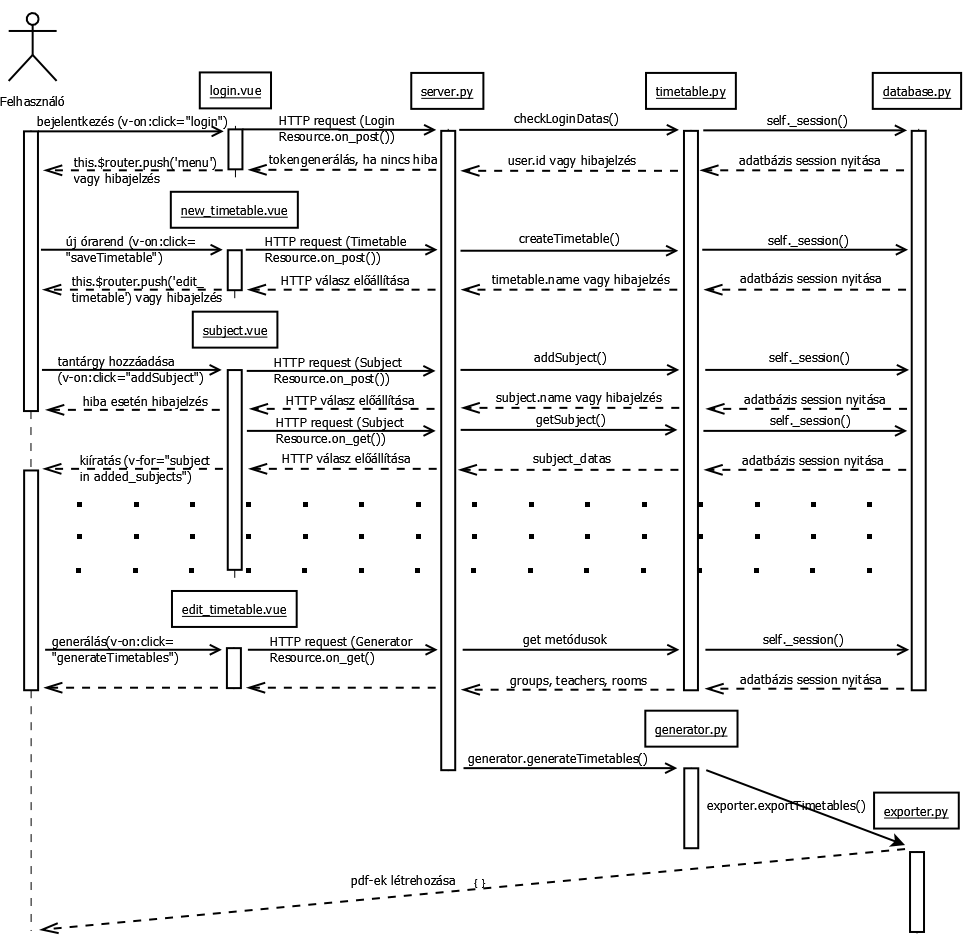
\includegraphics[width=\linewidth]{images/szekvencia.png}
	\caption{Az alkalmazás szekvenciadiagramja}
\end{figure}

\Section{Felhasználói dokumentáció}

A főoldal a \textit{login}, ahol bejelentkezésre van lehetőség, vagypedig ha még nem regisztráltunk vagy elfelejtettük a jelszavunkat, elérhetőek itt linkek, melyek az ezzel kapcsolatos oldalra irányítanak. Bejelentkezés után a menüben találjuk magunkat, ahol a fontos és egyben magyarázatra szoruló menüpontok, az Új órarend létrehozása és az Órarendjeim. Ha újat hozunk létre, meg kell adni a típust, hogy manuálisan akarjuk-e a tanárokat hozzárendelni az osztályokhoz, illetve hogy hány órától legyen a legkorábbi napi időablak és hány órakor érjen véget a legkésőbbi. Ezt a napi időintervallumot lesz lehetőség még szűkíteni a részmunkaidős tanárok esetében, az azonos nevű attribútumok állításával, tanár hozzáadásakor. A típus esetében általános iskola, középiskola és főiskola/egyetem közül választhatunk, ennek egyik jelentősége, hogy milyen típusú tantárgyakat lehet majd hozzáadni (pl. fakt típusú órák csak középiskolában vannak, elméletek és gyakorlatok pedig csak a főiskolán/egyetemen), a másik, hogy a főiskolán/egyetemen két óra hosszú egy időablak. Ha meglevő órarendet szeretnénk szerkeszteni, akkor kiválasztjuk melyiket szeretnénk és az abban a sorban található ceruza ikonra kattintunk (amennyiben törölni szeretnénk, akkor pedig nyilván a keresztre). Négy link fog megjelenni a számunkra, akkor is ha új órarendet hoztunk létre, akkor is ha meglevőt szerkesztünk. Egy a tantárgyak, egy a tantermek, egy a tanárok és egy az osztályok létrehozására. Új órarend esetén először mindenképpen tantárgyat/tantárgyakat kell hozzáadni, mert azzal kapcsolatban, hogy milyen tárgyai legyenek egy osztálynak, egy tanárnak, vagy hogy milyen tárgy(ak)ra legyen esetleg specializálódva egy terem, a korábban hozzáadottak közül választhatunk lenyíló listában. Ugyanígy, ha manuálisan rendeljük hozzá a tanárokat az osztályokhoz, csak a korábban hozzáadott tanárok közül választhatunk. Bármit is akarunk hozzáadni, egyszerre mindig egy példányt tudunk felvinni a megfelelő mezők kitöltésével (melyek elsősorban szövegmezők és lenyíló listák lesznek) és a hozzáadásra fenntartott nyomógomb lenyomásával. (Ez vonatkozik az osztály tantárgyainak hozzáadására is, osztály hozzáadásán belül.) Amint ez megtörtént, letárolódik az adatbázisban az adott objektum példány és a képernyő alján kiírásra is kerülnek a hozzáadott adatok, egyidejűleg alaphelyzetbe állnak a kitöltendő mezők és máris jöhet következő példány hozzáadása, ha szeretnénk. Mindez aszinkron, az oldal újratöltése nélkül történik. Ezenkívül van lehetőség törlésre, minden hozzáadott példánnyal kapcsolatban, a törlés ikonnal. Ha végeztünk a hozzáadásokkal és szeretnénk órarendet generáltatni, a Get it! gombra kell kattintani az \textit{edit\_timetable} oldalon. A felvitt adathalmaz méretétől függően sok időt is igénybe vehet az órarendgenerálás, de létre fog jönni az összes órarend pdf-jét tartalmazó mappa a fájlrendszer megadott helyén (ha publikussá tenném a webalkalmazást, akkor pedig letölthetővé válna az adott gép számára). Minden osztályé, minden tanáré és minden tanteremé külön pdf fájlban kap helyet, táblázatos formában. Bármikor van lehetőség újra generáltatni, akár ugyanazzal az adathalmazzal is. A véletlenszám-generálás miatt nem determinisztikus a folyamat, így változatlan adathalmaz esetén sem ugyanazokat a megoldásokat kapjuk újból, ha éppen nem elégedett az eredménnyel a felhasználó, próbálkozhat többször is. A \textit{my\_timetables} oldalról elérhetőek a meglevő adathalmazaink, a megfelelőt kiválasztva, a szerkesztés ikonra kattintva megintcsak az \textit{edit\_timetable} oldalon találhatjuk magunkat.

\Section{Tesztelés}

A szakdolgozat készítése során folyamatosan tesztelni kellett, azt lehet mondani, hogy a tesztelések a korábbi szakaszban az órarendgeneráló algoritmusokkal kapcsolatos tesztek voltak, a későbbi szakaszban pedig a webes működésekkel kapcsolatos tesztek. Az alábbiakban konkrétan megnevezem, milyen kritikus tényezőkre kellett különösen odafigyelni, illetve hol követtem el hibát.

Teremhozzárendelési feladat:
\begin{itemize}
	\item minden osztályhoz sikerült-e termet hozzárendelni
	\item speciális termet igénylő tárgyak esetén, más terem van-e az osztály-tantárgy kettősökhöz hozzárendelve, mint az osztályokhoz "alapból"
	\item egyes esetekben nem fér be tantárgy-specifikus terembe az osztály-tantárgy kettős, ilyenkor maradnia kell az osztálynak az alapból hozzárendelt teremben, mert valahol lenniük kell
\end{itemize}

Az időablakbeosztási feladat kapcsán biztosítani kellett, hogy amennyiben még van hely egy adott időablakban, de nincs több olyan osztály-tantárgy-terem-tanár hozzárendelés, amelyet  beoszthatnánk, akkor annak ellenére, hogy nem teljesen kitöltött az időablak, átlépjünk a következőbe. Ilyenkor keletkezhetnek lyukas órák, de ez elkerülhetetlen.

Genetikus algoritmus (időintervallum-hozzárendelési feladat):
\begin{itemize}
	\item a célfüggvényben megvizsgáltuk-e a tanárok előfordulásait az egyes időablakokban, vagy elkövettük azt a hibát, hogy csak az időablakok hossza (az időablakokban levő hozzárendelések száma) alapján számoltunk
	\item sikerült-e kiküszöbölni a korábban bemutatott keresztezési problematikát
	\item nem adtuk-e hozzá az új egyedeket a populációs listához, mielőtt a generáció összes egyedét kitenyésztettük, ugyanis ideiglenesen egy másik listában kell letárolni őket, mert az adott generációban született egyed még nem lehet szülő
\end{itemize}

Webes működések:
\begin{itemize}
	\item bejelentkezési ellenőrzésnél ne a jelszó eredeti formája és a hexadecimális kóddá konvertált kerüljön egymással összehasonlításra
	\item a hitelesítésekhez használt token benne maradt-e a HTTP kérelmekben
	\item lementődtek-e az adatbázisban a felvitt adatok, máskülönben esélytelen felhozni őket
	\item a több-több kapcsolatok megfelelően tárolódtak-e le, különös tekintettel az osztály-tantárgy kapcsolatokra, ahol a kapcsolótáblához kötődő attribútumok is vannak
	\item ha csak adott példányt vagy adott feltételnek eleget tevő példányokat akarunk felhozni,  rendben történik-e a paraméterátadás
	\item csak az adott órarenden belüli tantárgyak, tantermek, tanárok és osztályok kerülnek-e felhozásra, illetve csak az adott felhasználó órarendjei vannak-e meg
	\item a \textit{template.html} sablon megfelelő-e, különben nem fogja a kívánt tartalommal vagy egyáltalán tartalommal feltölteni a Jinja a html-eket
\end{itemize}

